\assignementTitle{Космический вальс}{30}{}

\textbf{Тренируемые навыки: }работа с массивами, рекурсивные алгоритмы перебора, школьный курс геометрии: расстояние между точками, параллельный перенос, зеркальное отражение, пересечение прямых, элементарная тригонометрия, работа с массивами и структурами данных.
\subsubsection*{Условие задачи}

Контрабандисты на корабле $A$ неожиданно подлетели к неподвижному патрульному кораблю $C$ по неизвестной сложной траектории. Патруль корабля $C$ попросил команду корабля $A$ предоставить запись маршрута движения с целью проверки посещения запретных зон. Однако, на корабле $A$ система записи маршрута движения не работала, и команда утверждала, что в запретные зоны они не заходили. Корабли могут двигаться только между узлами пятиугольной плитки, параметры которой и способ укладки приведены на рисунках 1 и 2. Командир $C$ обратил внимание на то, что команда $A$, как и команда $C$ слушает и записывает музыку радиостанции $B$. Сравнив мелодии, записанные на $A$ и $C$, командиру корабля $C$ удалось восстановить траекторию движения корабля $A$ и проверить контрабандистов.

Вам предлагается решить эту же задачу — определить траекторию движения корабля $А$, сравнив записи мелодий на кораблях $А$ и $C$. Радиостанция находится в начале системы координат, т.е. $x_B=y_B=0.0$. Данные передаются и принимаются пакетами длительностью в ♪$=1/8$. Каждый пакет представляют собой отдельную строку в текстовом файле, хранящем запись мелодии. Каждый пакет передается и принимается, во время движения корабля от вершины к вершине. Пример мелодии и соответствующий ей файл приведены ниже в приложении А.


\begin{tabular}{p{7cm}p{7cm}}
    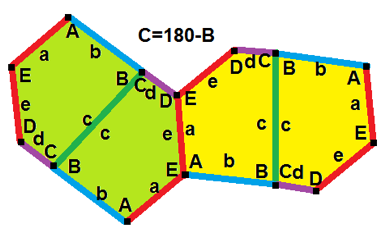
\includegraphics{2}

    Рисунок 1. $a = e, B + C = 180^\circ, A + D + E = 360^\circ$ & 
    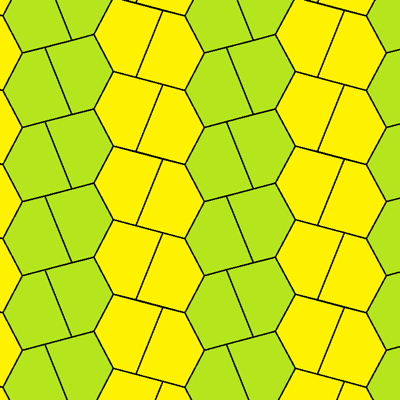
\includegraphics{1}

    Рисунок 2. Способ замощения пространства.
        
\end{tabular}

Постоянные параметры задачи:
\begin{itemize}
    \item Скорость распространения сигнала $С = 100000.0$ (сигнал распространяется по прямой, не по вершинам);
    \item Скорость корабля $V = 250.0$;
    \item Несущая частота $f_0= 40000.0$.
\end{itemize}

\inputfmtSection


Input.dat
\begin{itemize} 
    \item Координата корабля $А\space \{x_A,y_A\}$, 
    \item координата корабля $С\space \{x_C,y_C\}$, 
    \item координаты вершин трех плиток, окружающих точку $В$,
\end{itemize} 
Real\_song.dat — переданный файл с корабля В, 
Record\_song.dat — Принятый файл на корабле А.


\outputfmtSection

Output.dat — файл с маршрутом движения (последовательность координат узлов, посещенные корабле А до встречи с патрульным кораблем В).

Формат Output.dat:

КоординатаX	КоординатаY	Доплеровское смещение частоты

\markSection

Задача считается решенной, если суммарное отклонение найденной траектории от действительной траектории А не превышает 10\% от общей длины маршрута.

Проверка проводилась в несколько этапов(попыток), проводимых в заданную дату (20.12.2018; 29.12.2018;06.01.2019; 11.01.2019; 14.01.2019). В каждой попытке участники могли загрузить и проверить одно свое решение этой задачи.

Результирующая оценка за задачу выбиралась, как максимальная из попыток.

Загрузка решений проводилась на сайте \url{http://dep1.iszf.irk.ru/wlcomm} на котором было установлено специальное программное обеспечение для регистрации, разделения доступа и возможности загрузки решений участниками.

Тестирование решений проводилось на виртуальной машине с установленной ОС Kubuntu, проверку и начисление баллов за каждый тест осуществляли автоматические программы.

\subsection*{Приложение А}

Таблица нот и соответствующих им частот в Гц.

\putImgWOCaption{16cm}{7}

Мелодию будем представлять в текстовом формате, следующего вида. Например, на нужно закодировать первую строку в мелодии «Танец утят»:
\putImgWOCaption{16cm}{4}

В строках будем отмечать ноты длительностью 1/8, если нота прерывается то ставим 2, если нота продолжает звучать ставим 1, например:

\putImgWOCaption{16cm}{5}

Мелодии, записанные на кораблях А и С отличаются, так как корабль С остается неподвижным, а корабль А двигается. В этом случае на А наблюдается эффект Доплера – изменение частоты излучения, воспринимаемое наблюдателем (приёмником), вследствие движения источника излучения и/или движения наблюдателя (приёмника). Смещение частоты $df$ можно найти по следующей формуле:
$$df=\frac{f_0 V_r}{C}.$$

Например, угол между радиус-вектором $R$ и вектором скорости $V$ составляет 60 град, тогда радиальная скорость $V_r = 250 \cdot cos(60) = 125$ и $df = 50$ Гц. Если в этот момент передавалась нота Ля первой октавы (частотой 440 Гц), тогда на корабле А ее услышали на частоте $440+50=490$ Гц, так как приемник записывает только «чистые» ноты, то была записана наиболее близкая к 490 Гц нота Си (первой октавы, частота $493.88$ Гц.)

\putImgWOCaption{7cm}{6}

Для вычисления доплеровского смещения частоты необходимо найти радиальную скорость $V_r$ – проекцию скорости движения $V$ на радиус вектор $R$, направленный от А к В.

Проверка проводилась в несколько этапов(попыток), проводимых в заданную дату (20.12.2018; 29.12.2018; 06.01.2019; 11.01.2019; 14.01.2019). В каждой попытке участники могли загрузить и проверить одно свое решение этой задачи.

Результирующая оценка за задачу выбиралась, как максимальная из попыток.

Загрузка решений проводилась на сайте \url{http://dep1.iszf.irk.ru/wlcomm} на котором было установлено специальное программное обеспечение для регистрации, разделения доступа и возможности загрузки решений участниками.

Тестирование решений проводилось на виртуальной машине с установленной ОС Kubuntu, проверку и начисление баллов за каждый тест осуществляли автоматические программы.

\subsection*{Алгоритм решения задачи}

\begin{enumerate}
    \item Так как известны координаты вершин трех базовых плиток решетки вокруг начала координат, то построить решетку можно с помощью параллельных переносов и зеркальных отражений.
    \item На полученной решетке построение требуемой траектории можно с помощью небольшой модификации стандартного переборного алгоритма (\url{http://acm.mipt.ru/twiki/bin/view/Algorithms/GenerateCPP}). Модификация заключается в том, что выход из рекурсии происходит на «запрещенных» вершинах, т.е. таких вершинах переход в которые запрещен доплеровским сдвигом частоты (формула приведена в условии).
\end{enumerate}